\subsubsection{Login}
\textbf{Steps}
\begin{itemize}
    \item Open the website from the Url.
    \item Enter the Manager username and password.
    \item Click Login
\end{itemize}
\begin{figure}[H]
    \centering
    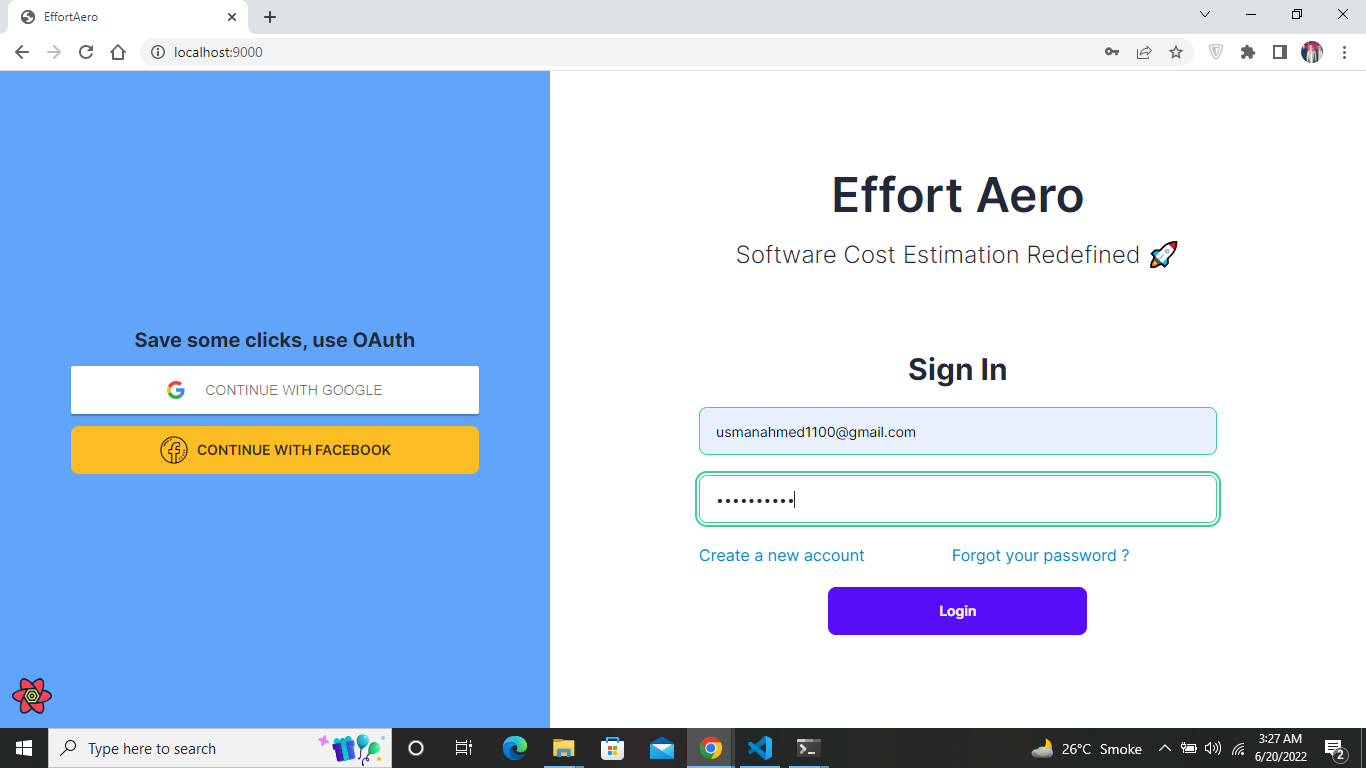
\includegraphics[scale=0.4]{./diagrams/user-manual/Screenshot (17).png}
    \caption{User manual of Login}
    \label{fig:user-1}

\end{figure}
%image of the login page

\subsubsection{Dashboard}
\textbf{Steps}
\begin{itemize}
    \item After Login, you will be redirected to the Dashboard.
    \item From Dashboard of Manager you can see the list i.e Organization, projects, Stats, etc.
    \item First You see the Create Organization button and Organization List.
    \item Click on the Create Organization button to create a new Organization.
    \item Click on List of Organization, projects, Stats, etc. then you can redirected to the respective page.
\end{itemize}

\begin{figure}[H]
    \centering
    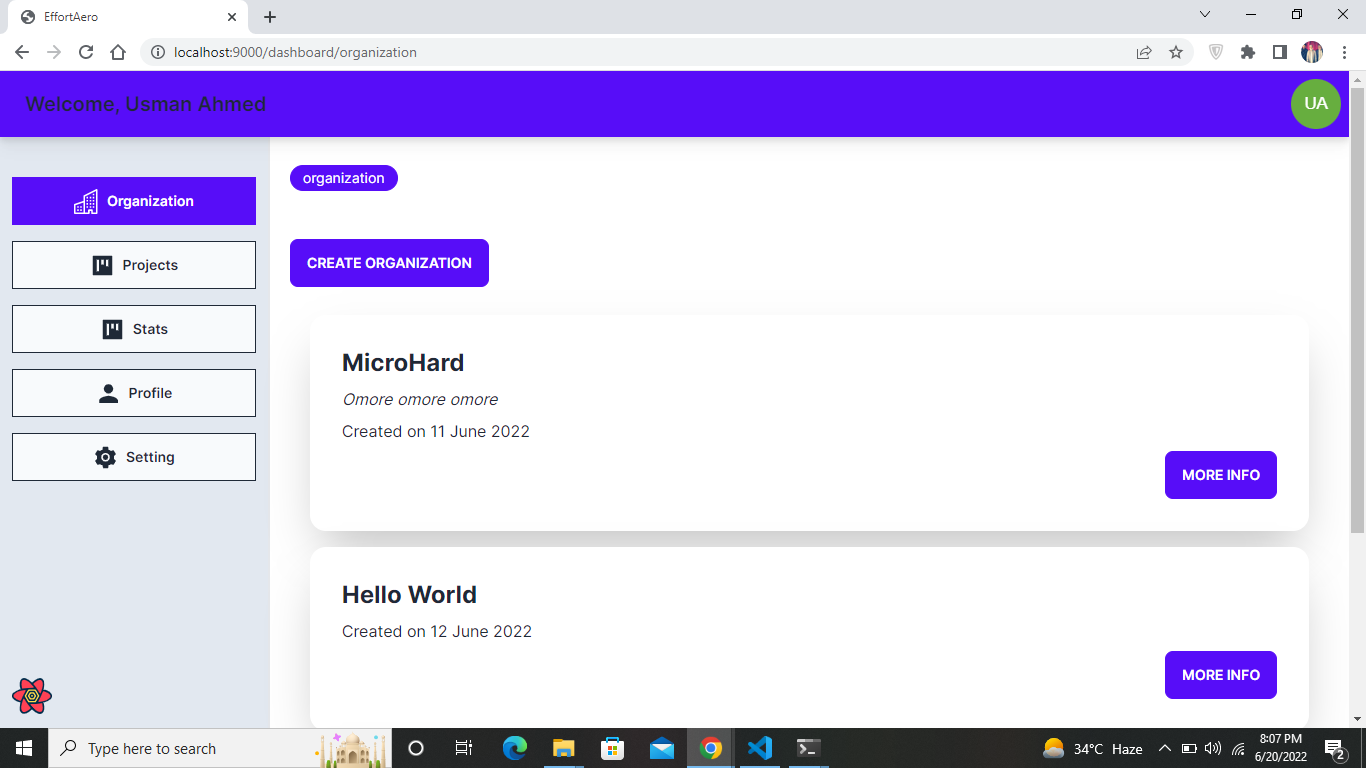
\includegraphics[scale=0.4]{./diagrams/user-manual/Screenshot (18).png}
    \caption{User manual of Dashboard}
    \label{fig:user-1}

\end{figure}

\subsubsection{Organization Information}
\textbf{Steps}
\begin{itemize}
    \item After Click on More Info Button located on the right bottom corner of the Organization tile, you will see the Organization Information.
    \item On the page, you can see the name of the Organization, Date of creation, Oraganization's Member portion, and organzaition project's portion.
    \item In the Organization Member portion, you can see the list of the members of the Organization with a Search bar to search for a member to add in the organization projects.
    \item In the Organization Project portion, you can see the list of the projects of the Organization with delete and info button.
    \item From info button, you can see the project's information.
    \item From delete button, you can delete the project from the organization.
\end{itemize}

\begin{figure}[H]
    \centering
    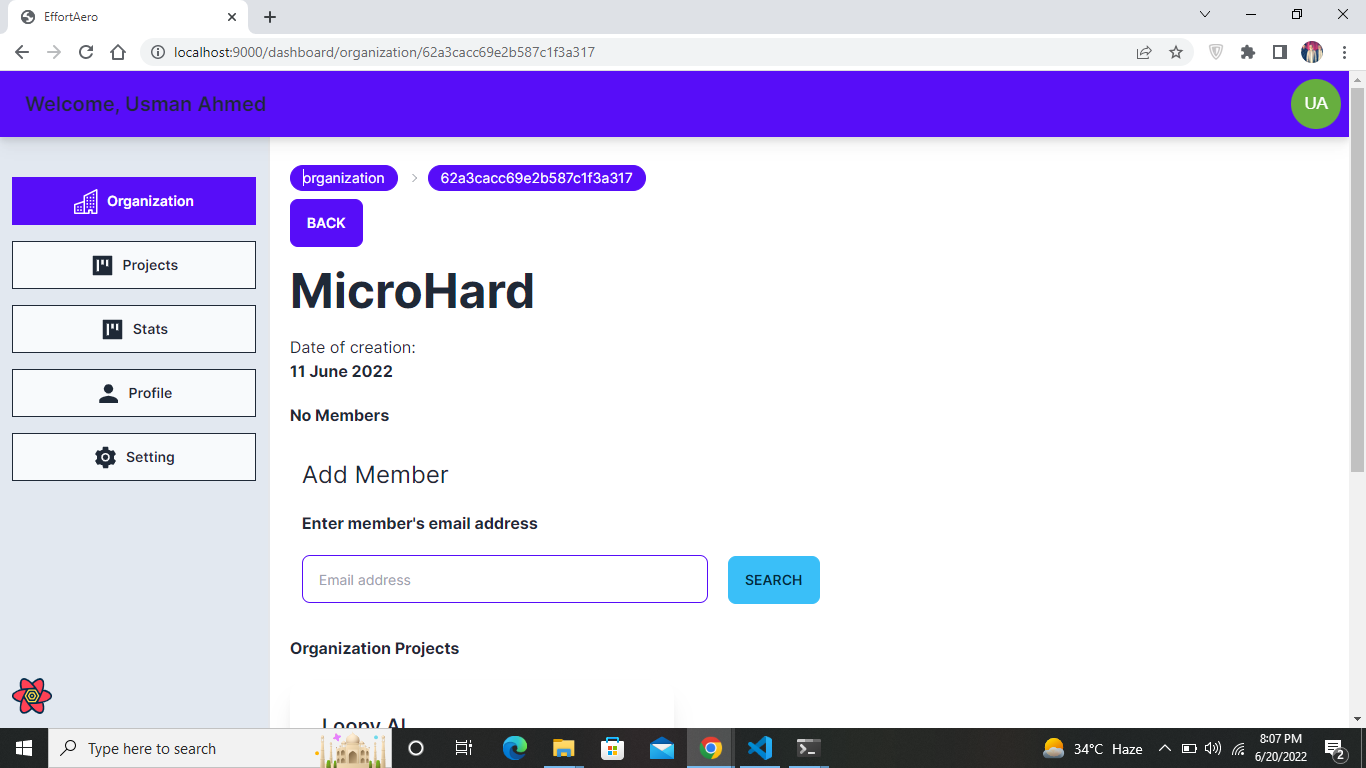
\includegraphics[scale=0.4]{./diagrams/user-manual/Screenshot (20).png}
    \caption{User manual of Oraganization Information}
    \label{fig:user-1}
\end{figure}

\begin{figure}[H]
    \centering
    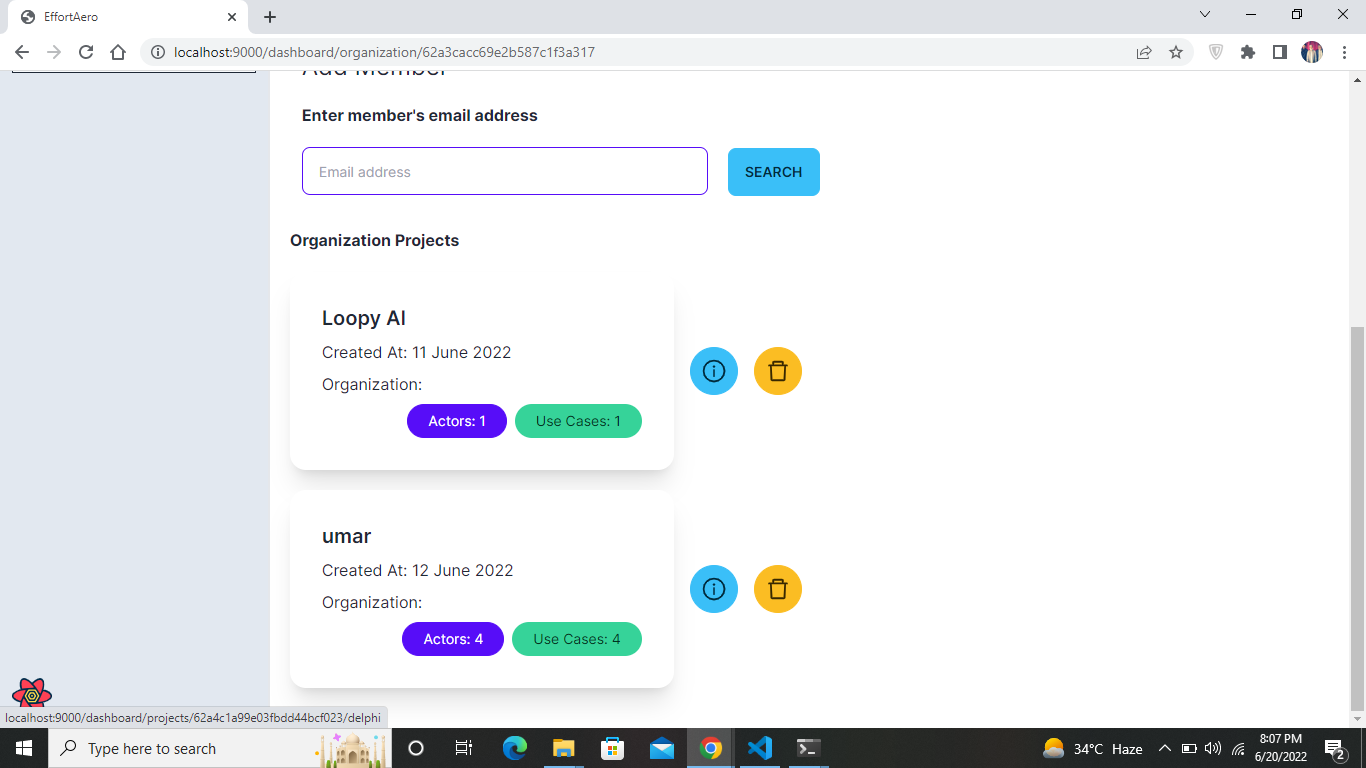
\includegraphics[scale=0.4]{./diagrams/user-manual/Screenshot (21).png}
    \caption{User manual of Organization Information 2}
    \label{fig:user-1}

\end{figure}


\subsubsection{Project Information}
\textbf{Steps}
\begin{itemize}
    \item After Click on info Button located on the right of the Project tile, you will see the Organization Information.
    \item On the page, you can see the name of the Project, Project's Organization , calculate estimate and project attribute portion.
    \item In project attribute portion, you can see the list of the attributes of the project with two button one is Update Attribute Button and second is Download Atributes.
    \item From Update Attribute Button, you can update the attribute of the project.
    \item From Download Attribute Button, you can download the attribute of the project.

\end{itemize}

\begin{figure}[H]
    \centering
    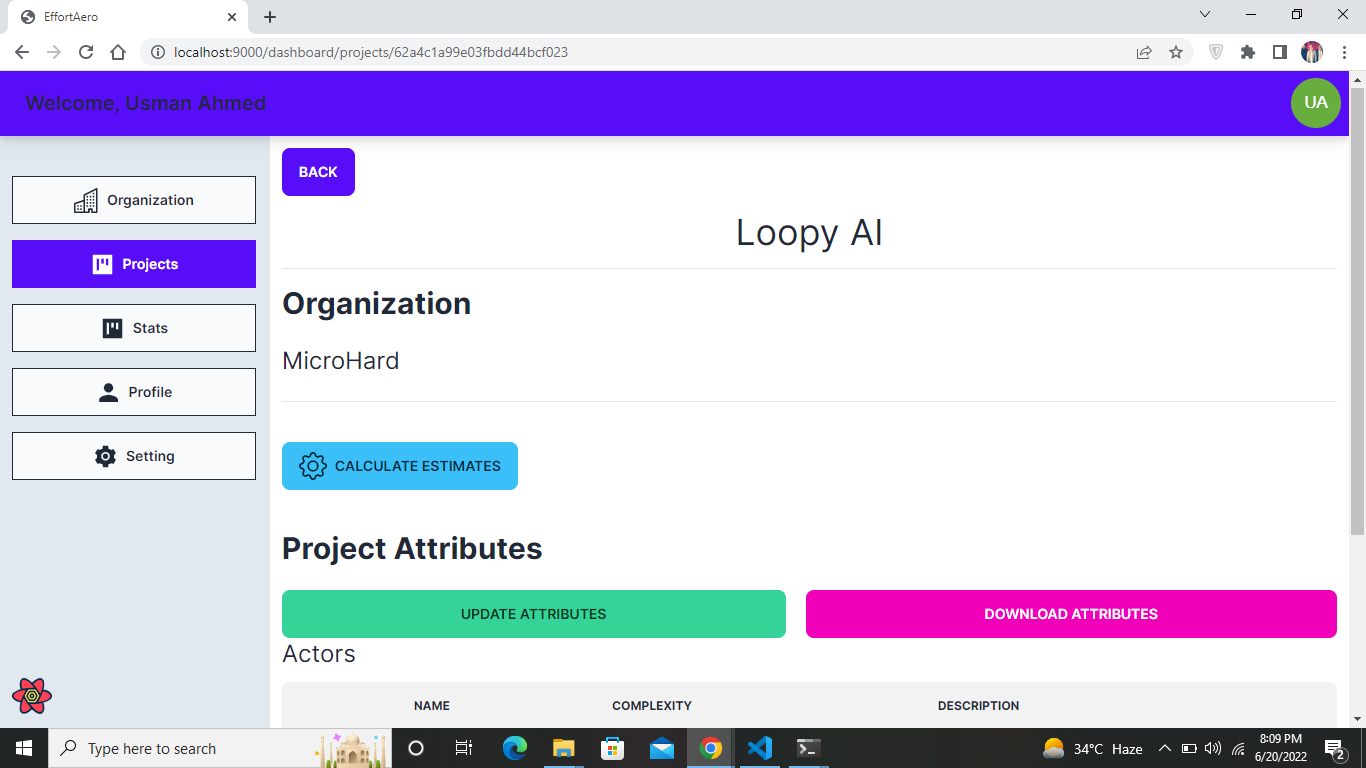
\includegraphics[scale=0.4]{./diagrams/user-manual/Screenshot (30).png}
    \caption{User manual of Project Info}
    \label{fig:user-1}

\end{figure}

\begin{figure}[H]
    \centering
    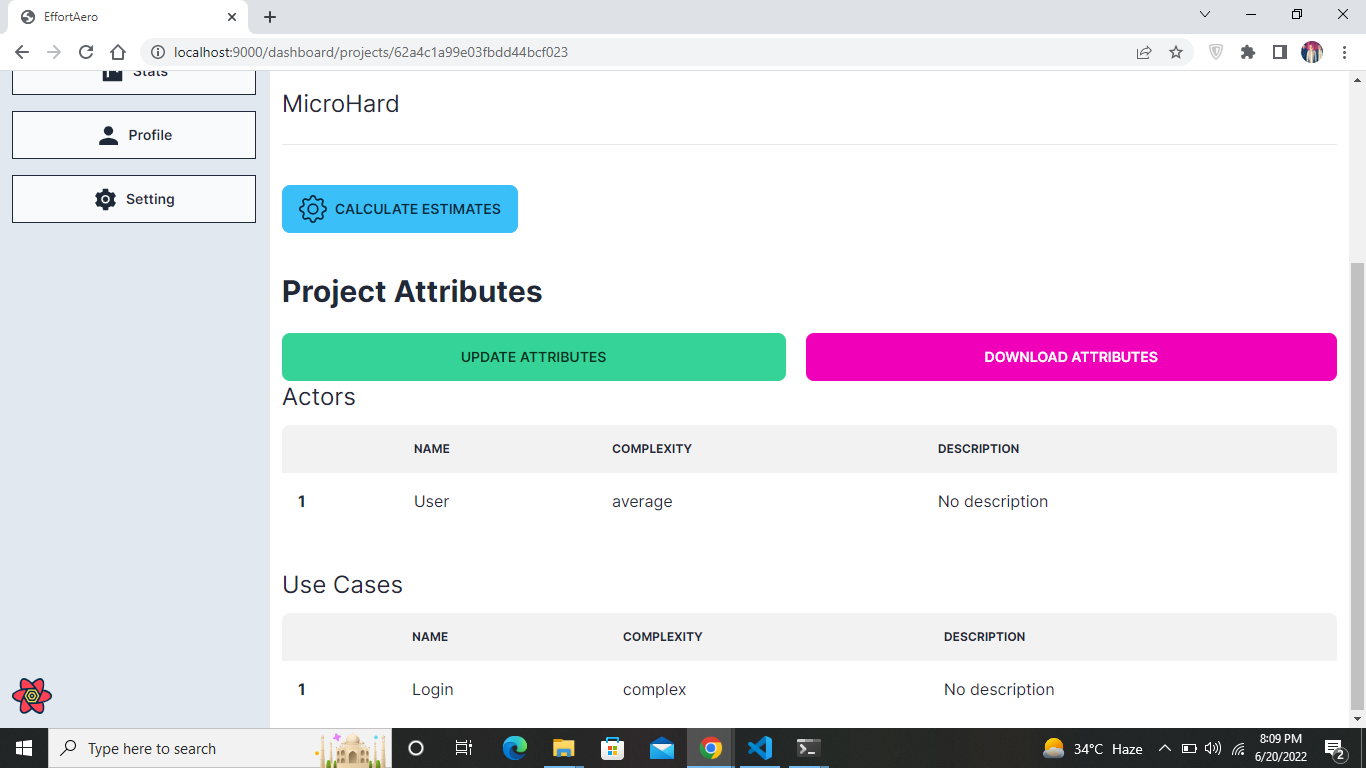
\includegraphics[scale=0.4]{./diagrams/user-manual/Screenshot (31).png}
    \caption{User manual of Project Info}
    \label{fig:user-1}

\end{figure}

\subsubsection{Calculate Estimate}
\textbf{Steps}
\begin{itemize}
    \item After Click on Calculate Estimate Button, you will see different methods to calculate the estimate.
    \item In Estmation List, we have 4 methods to calculate the estimation.
    \item First Method is UCP (User Case Points) Calculation in which you have request for estimation on the bases of use case point formula.
    \item Second Method is Delphi Technique, in which you have request to the developer for estimation on the bases of their experience.
    \item Third Method is Machine Learning Technique, in which machine learning module estimate the estimation on the bases of the previous data.
    \item Fourth Method is Esembled Method which is the combination of all the above methods.
\end{itemize}

\begin{figure}[H]
    \centering
    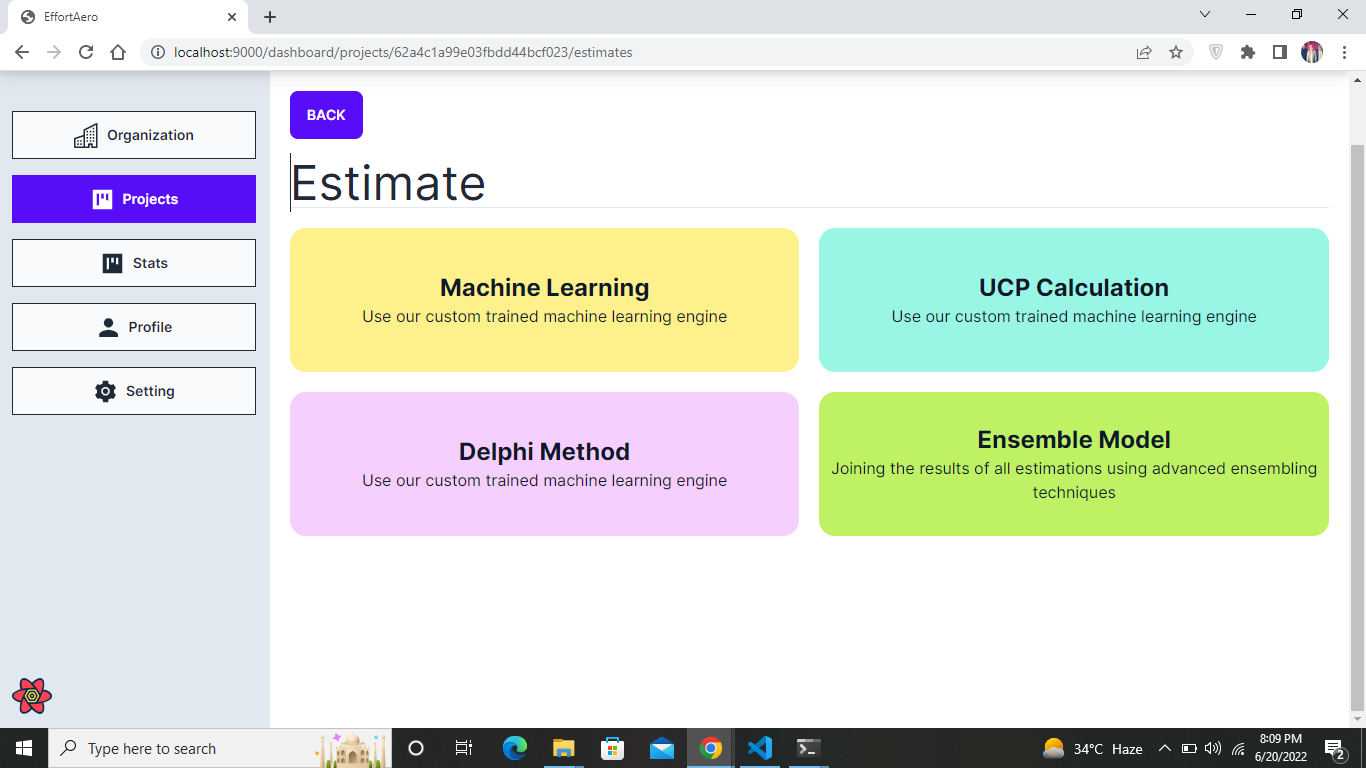
\includegraphics[scale=0.4]{./diagrams/user-manual/Screenshot (32).png}
    \caption{User Manual of Calculate Estimate}
    \label{fig:user-1}

\end{figure}

\begin{figure}[H]
    \centering
    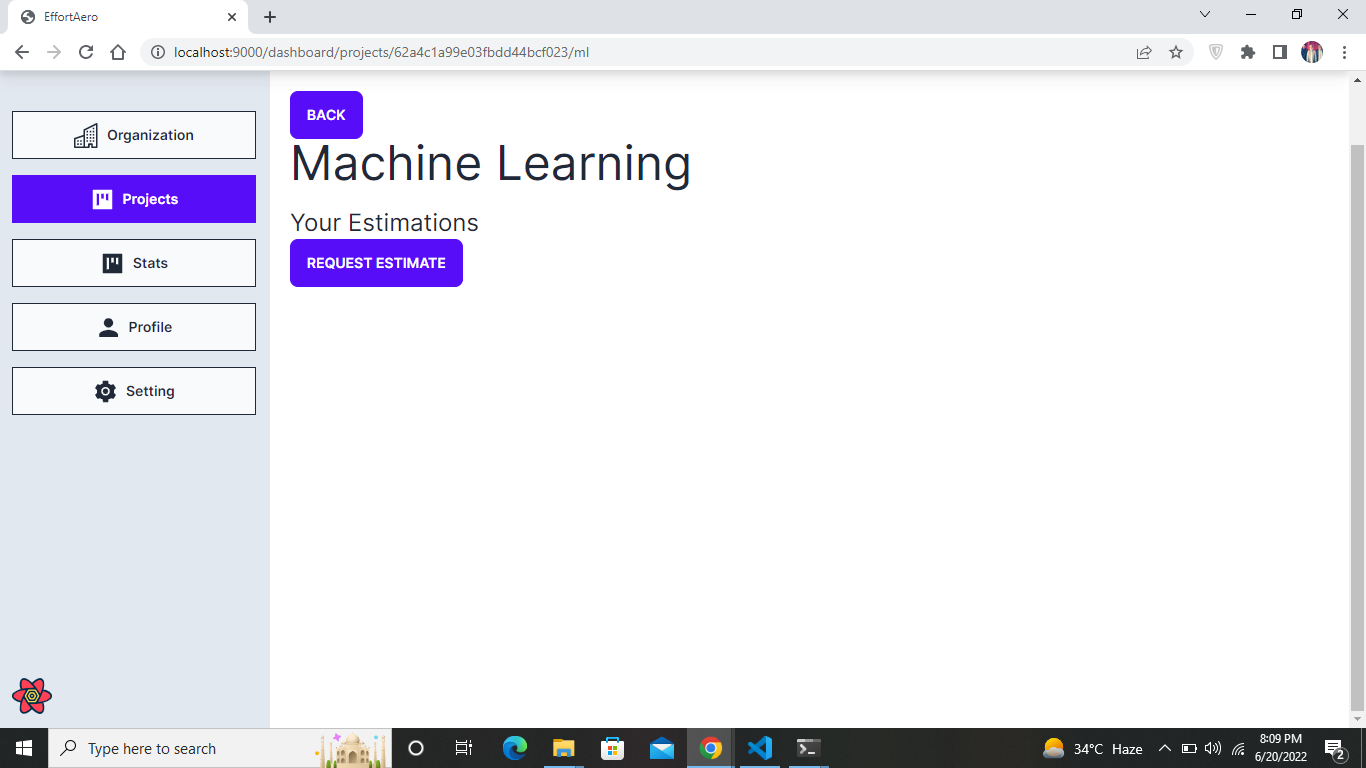
\includegraphics[scale=0.4]{./diagrams/user-manual/Screenshot (33).png}
    \caption{User Manual of Machine Learning}
    \label{fig:user-1}

\end{figure}

\begin{figure}[H]
    \centering
    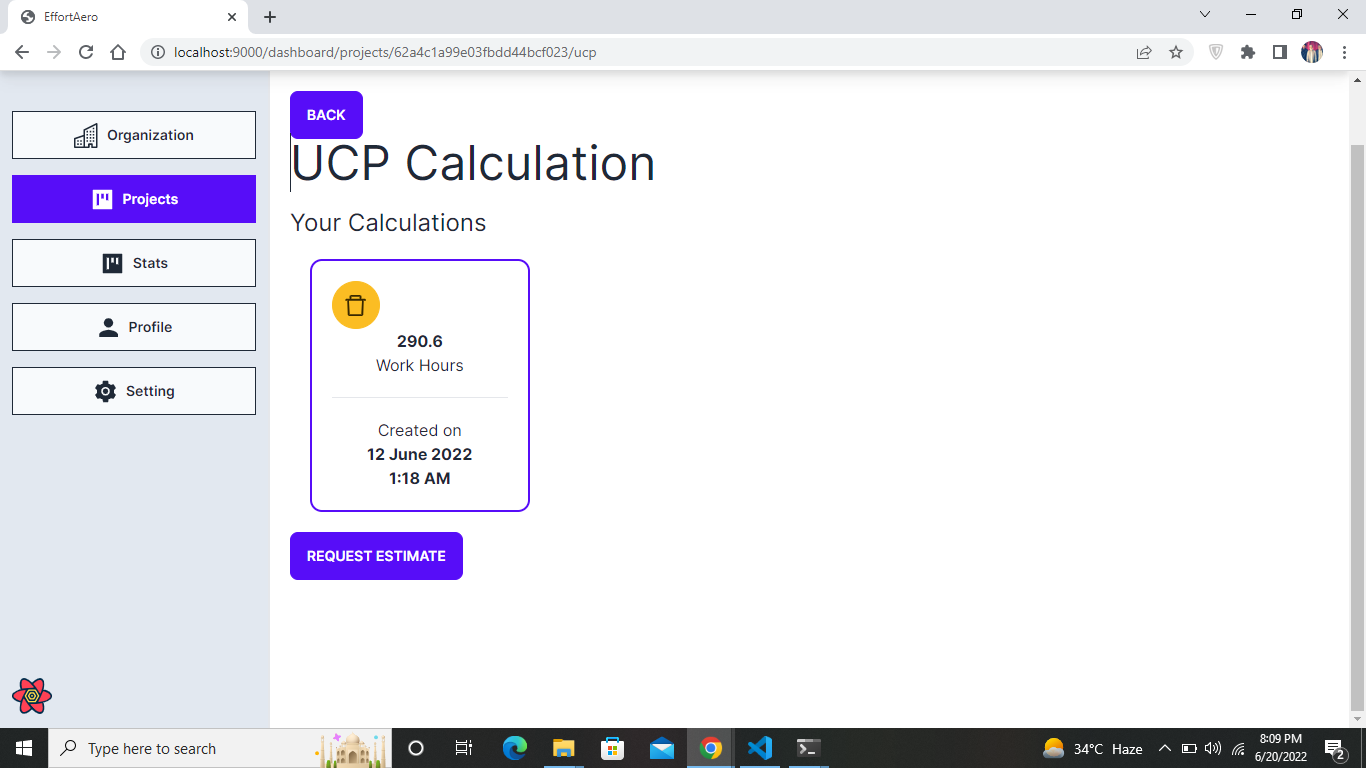
\includegraphics[scale=0.4]{./diagrams/user-manual/Screenshot (34).png}
    \caption{User manual of UCP Calculation}
    \label{fig:user-1}

\end{figure}

\begin{figure}[H]
    \centering
    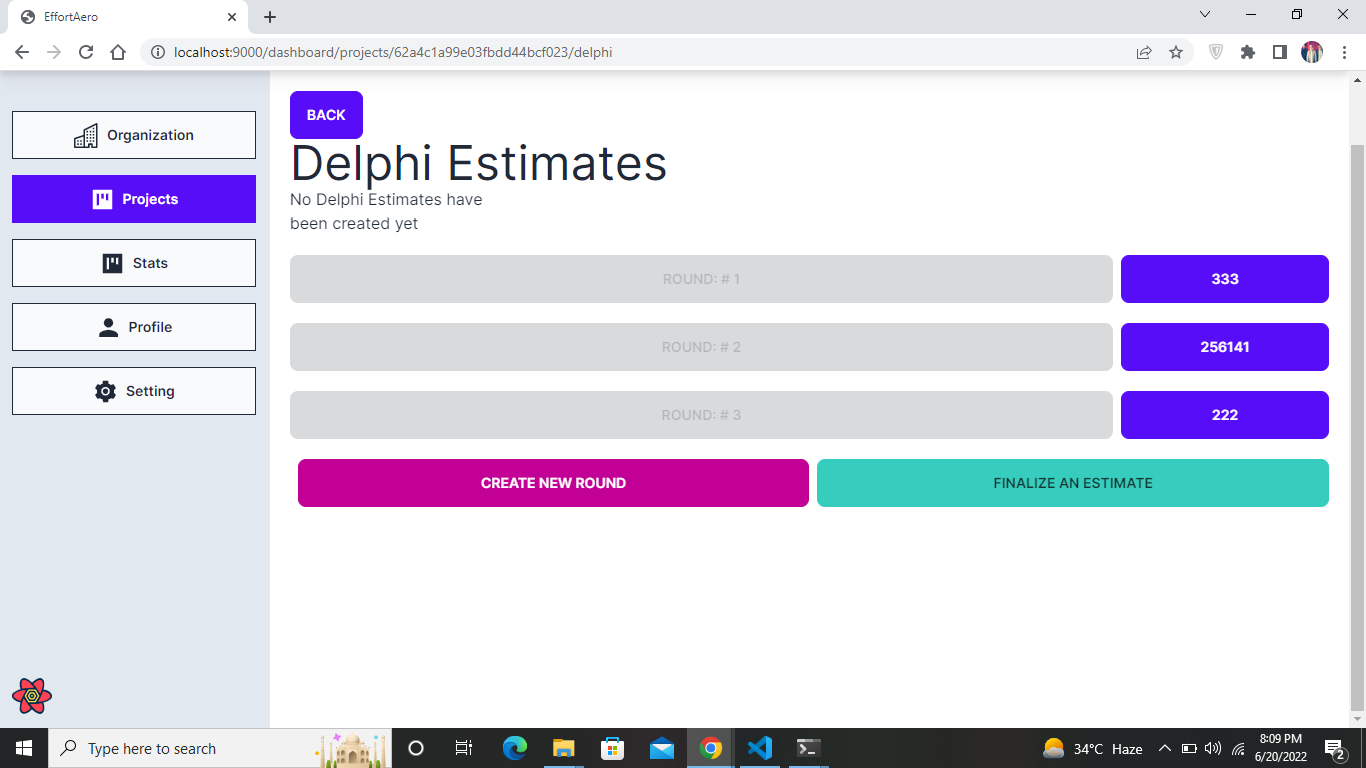
\includegraphics[scale=0.4]{./diagrams/user-manual/Screenshot (35).png}
    \caption{User manual of Delphi Technique}
    \label{fig:user-1}

\end{figure}

\begin{figure}[H]
    \centering
    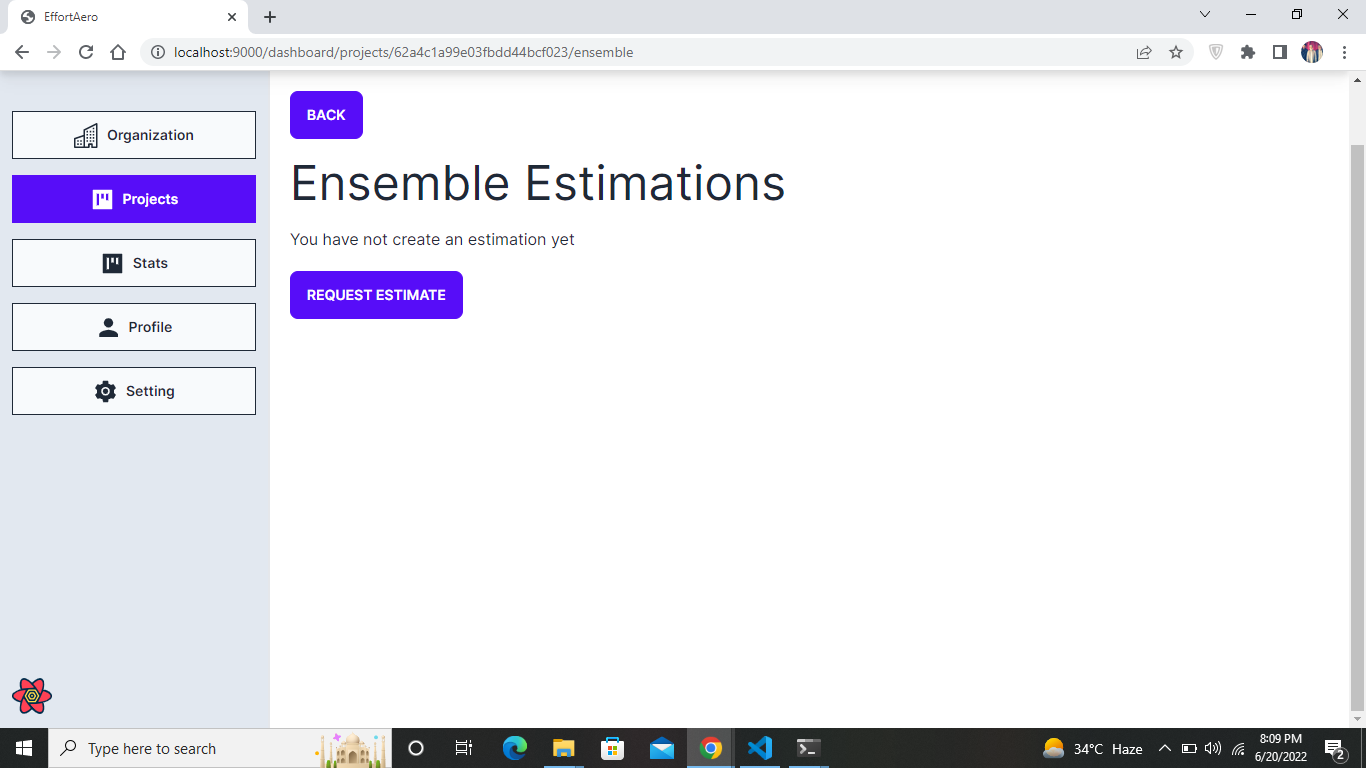
\includegraphics[scale=0.4]{./diagrams/user-manual/Screenshot (36).png}
    \caption{User manual of Esembled Module }
    \label{fig:user-1}

\end{figure}

\subsubsection{Stats}
\textbf{Steps}
\begin{itemize}
    \item  After Click on Stats Button, you will see the list of stats of the Projects.
    \item  In the list, you can see the list of the projects with their projects attributes.
    \item  When you click on the project, you will see the project's Estimation Stats.
    \item  In the Estimation Stats, you can see the list of the Graph of the project with their respective estimation.
\end{itemize}

\begin{figure}[H]
    \centering
    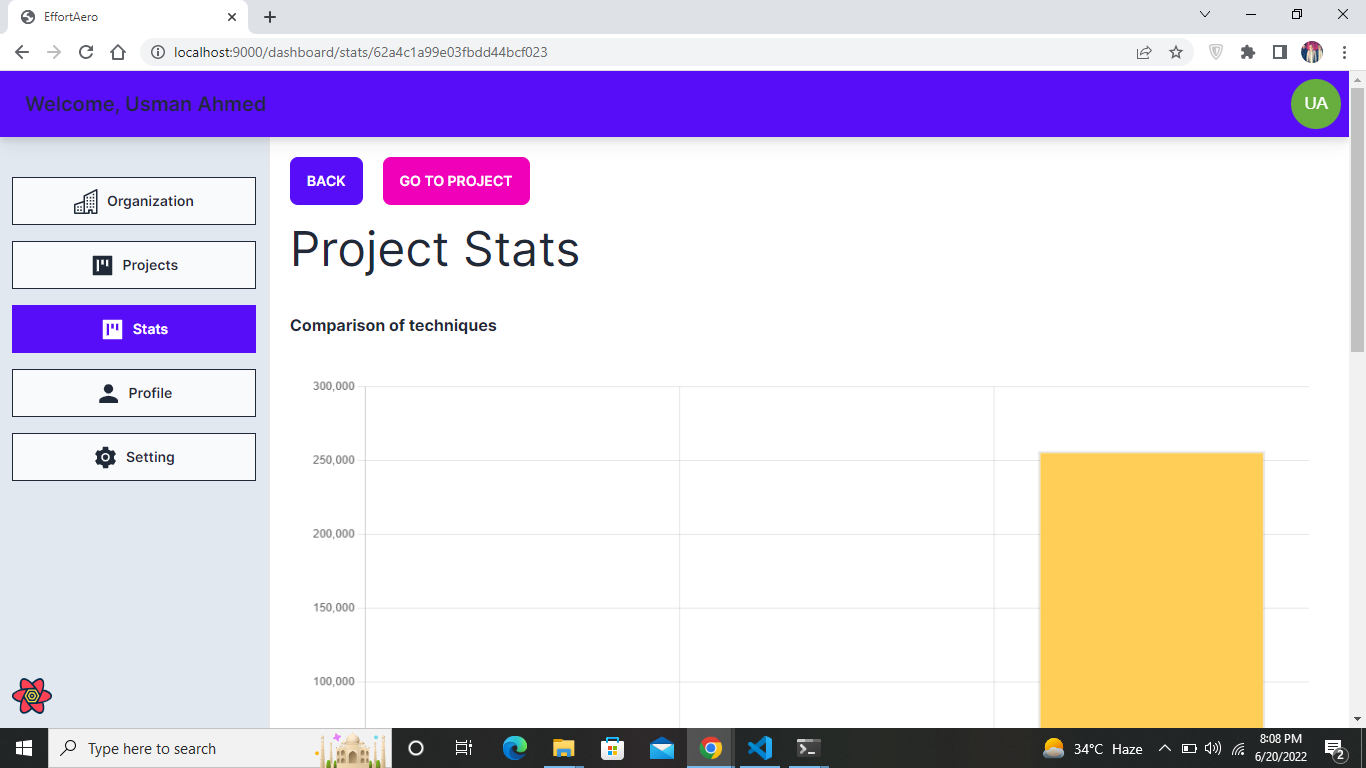
\includegraphics[scale=0.4]{./diagrams/user-manual/Screenshot (26).png}
    \caption{User manual of Stats of Project}
    \label{fig:user-1}

\end{figure}

\begin{figure}[H]
    \centering
    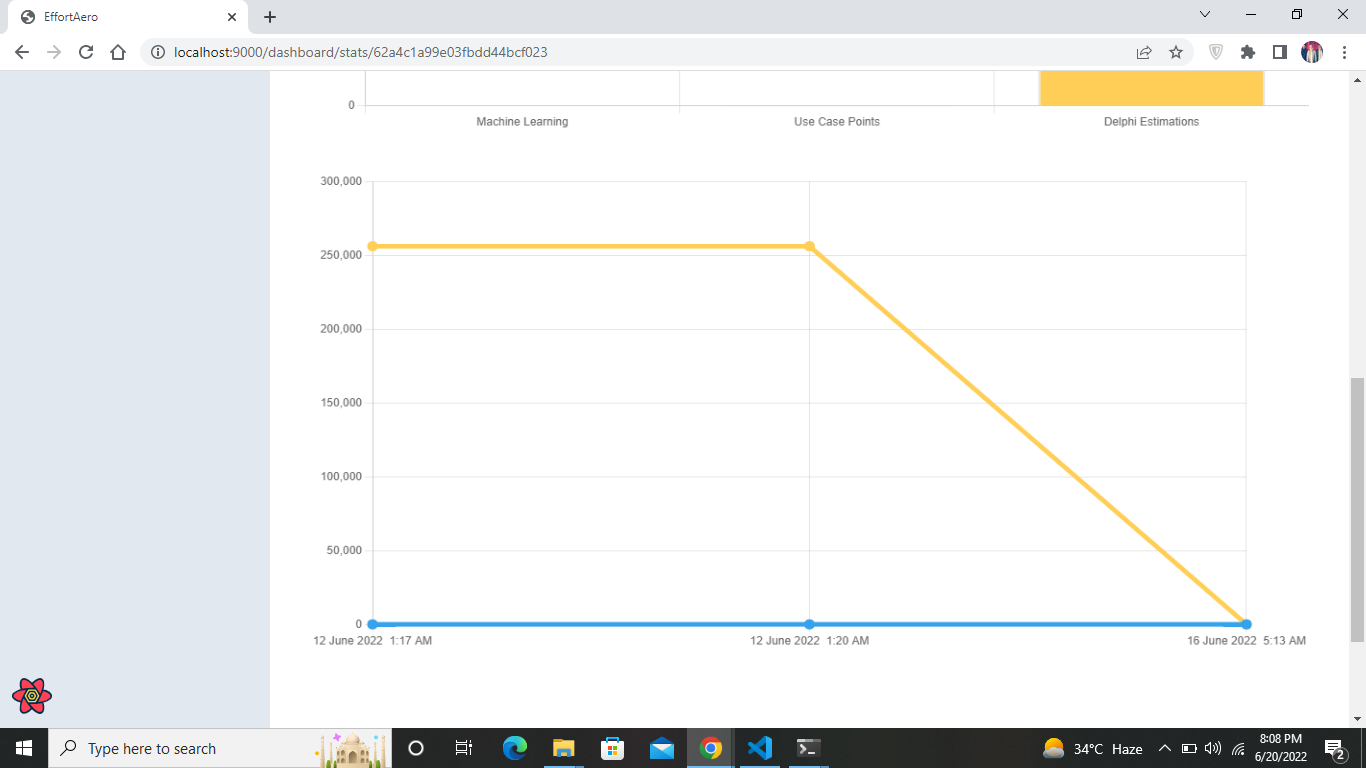
\includegraphics[scale=0.4]{./diagrams/user-manual/Screenshot (27).png}
    \caption{User manual of Stats of Project 2}
    \label{fig:user-1}

\end{figure}

\subsubsection{Profile}
\textbf{Steps}
\begin{itemize}
    \item In Profile Page, you can see the profile of the user.
    \item You can change the name of the user.
    \item You can change the password of the user.
    \item You can change the email of the user.
    \item Then clicked on Update Changes Button to update the changes.

\end{itemize}

\begin{figure}[H]
    \centering
    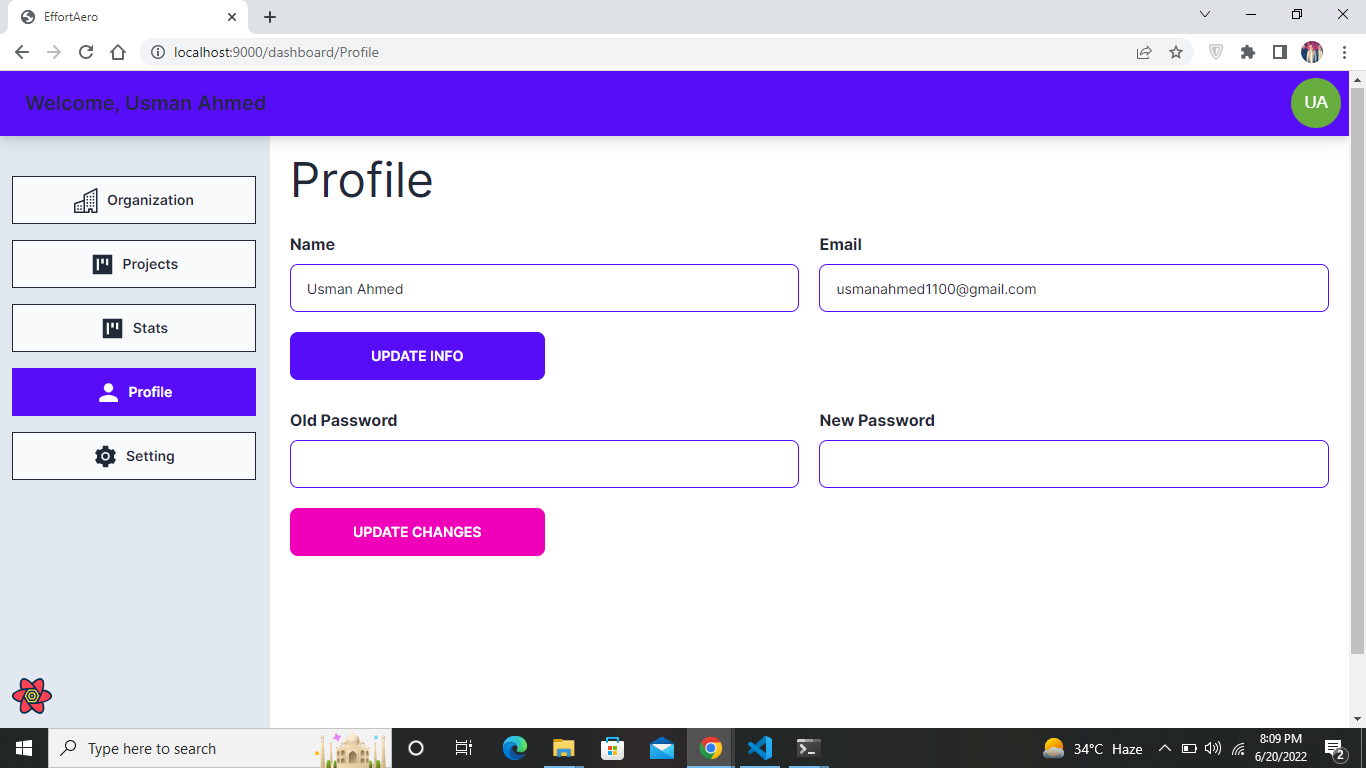
\includegraphics[scale=0.4]{./diagrams/user-manual/Screenshot (28).png}
    \caption{User Manual of Profile Page}
    \label{fig:user-1}

\end{figure}

\subsubsection{Setting}
\textbf{Steps}
\begin{itemize}
    \item After Click on Setting Button, you will see the Setting Page.
    \item In Setting Page, you can change the theme of the application.
    \item With the change of theme, you can see the logout button as well.
\end{itemize}

\begin{figure}[H]
    \centering
    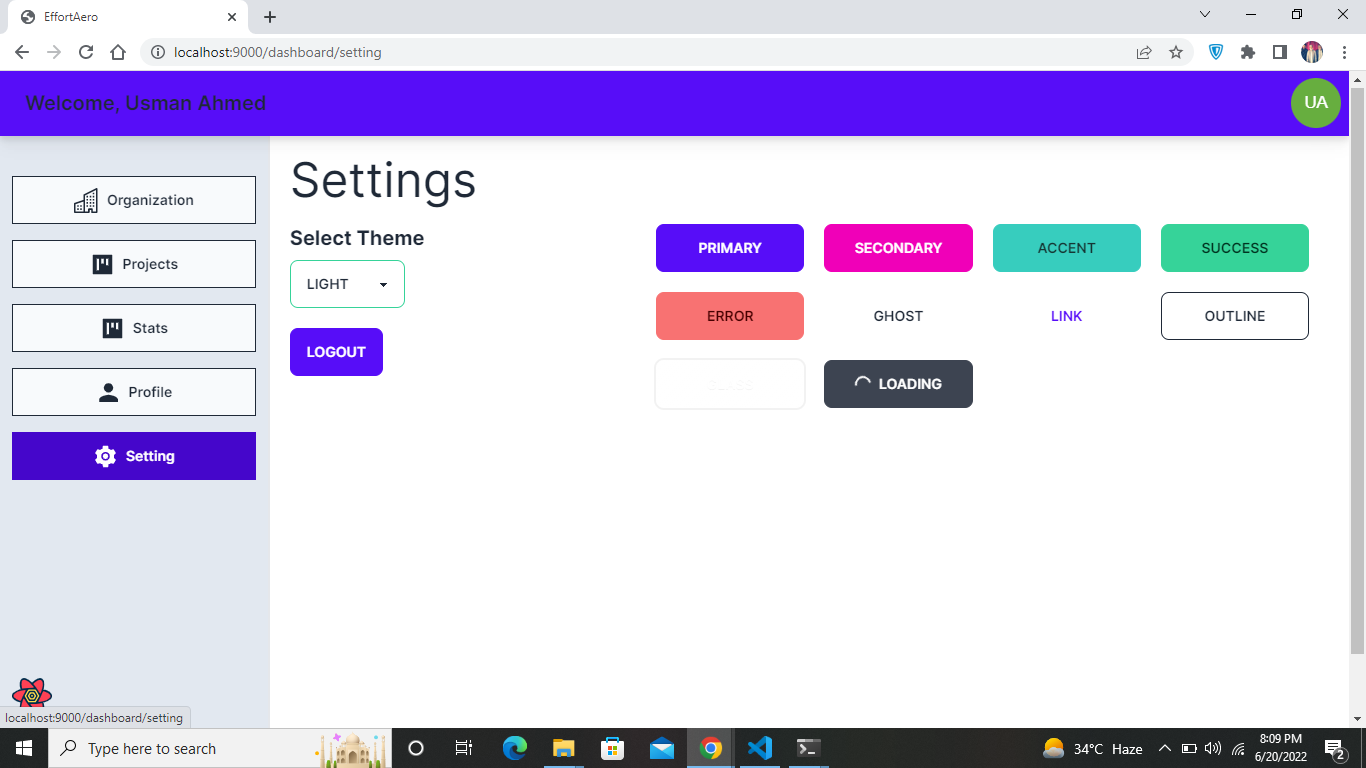
\includegraphics[scale=0.4]{./diagrams/user-manual/Screenshot (29).png}
    \caption{User manual of Setting Page}
    \label{fig:user-1}

\end{figure}
